\documentclass{article}

\usepackage[a4paper, total={15cm, 24.5cm}]{geometry}
\usepackage{float}
\usepackage{amsfonts}
\usepackage{graphicx}
\usepackage{amsmath}
\usepackage{array}
\usepackage{multicol}

\title{Foundations of Operations Research}
\author{Elia Ravella}
\begin{document}
	\begin{titlepage}
		\maketitle
	\end{titlepage}
	
	\tableofcontents
	\clearpage

	\section{Graphs}
		\subsection{Definitions}
			A graph is a pair of sets. Graph $G = (N, E)$ is composed of a set N of nodes and a set E of edges, that are themselves pair of nodes. The intuitive representation is the classic web of interconnected nodes.\\
			Two nodes are said to be \textit{adjacent} if there's an edge connecting them.\\
			An edge is \textit{incident} to a node if it has that node at an endpoint.\\
			The \textit{degree} of a node is the number of incident edges to it.\\
			A \textit{path} is a subset of the E set composed of consecutive edges (the endpoint of an edge is the "start"point of the next one\footnote{not in a directional way: we are still talking about non directed graphs, the two consecutive edges just in fact share an endpoint}) that connects some edges in the graph.\\
			Two nodes are \textit{connected} if exists a path that links them. A graph con be \textit{connected} to, if and only if there exists a path the connects \textbf{all its nodes}.\\
			A graph is \textit{directed} if some of the edges can be traversed in only one way. These edges are called \textit{arcs}.\\
			A \textit{cycle} or \textit{circuit} is a directed path that end where it starts.\\
			A graph is \textit{complete} if for all pair of nodes there's an edge connecting them. Reasoning on this line, we can define the upper bounds for the number of edges given the nodes:
			\begin{equation}
				\begin{cases}
					e \leq \frac{n \times (n-1)}{2} \text{ if undirected} \\
					e \leq n \times (n-1) \text{ if directed}
				\end{cases}
			\end{equation}
			where intuitively "e" is the number of edges and "n" the number of nodes. Given this two inequalities, we can redefine completeness: a graph is complete if and only if $e = \frac{n \times (n - 1)}{2}$ or $e = n \times (n - 1)$ depending on the graph being directed.

			\paragraph{Cuts}
				Given an undirected graph $G = (N, E)$ we can take $S \subset G$ subsets of nodes; we then observe $\delta(S)$ the \textit{cut} induced by S is the subsets of \textbf{edges} that connects S to N \textbackslash S.
				\begin{figure}[H]
					\centering
					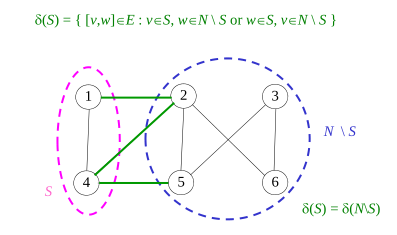
\includegraphics[width = \textwidth]{./images/Cut.png}
				\end{figure}
				Same definition holds for directed graphs, but this time we can distinguish among \textit{outgoing} and \textit{incoming} cuts, wheter the edges are all exiting S or ending in it.\\
				A graph is said to be \textit{bipartite} if we find a partition $N = (N_1, N_2)$ such as $\delta(N_i) = \emptyset$. So \textbf{the two subsets are disconnected}.\\
				A bit of foreshadowing: if a cut from a partial tree to another portion of the graph holds a minimum cost arc, then \textit{there exists a spanning tree with that arc}. This is called the cut property.
				
			\paragraph{Data Representations for Graphs}
			Depending one the edges / nodes ratio, two different data structures can hold a valid representation for a graph. When $e \approx n^2$ (a dense graph) then an adjacency matrix is the best choice. Otherwise (sparse graphs) linked lists of successors for each node.  

		\subsection{Reachability}
			The reachability problem can be formulated as "given a graph, determine all the nodes that are reachable from a starting one, decided a priori. A node is reachable is there's a path from the starting one and itself".

		\subsection{Subgraphs, Trees, Spanning Trees}
			We call $G' = (N', E')$ a subgraph of $G = (N, E)$ if and only if
			\begin{equation}
				\begin{cases}
					N' \subseteq N \\
					E' \subseteq E \\
					\text{all edges inside $E'$ connects nodes in $N'$}
				\end{cases}
			\end{equation}
			A \textit{tree} $G_t = (N', E')$ is a subgraph of a network that's both \textbf{connected} and \textbf{acyclic}. A tree is \textit{spanning} if it contains all the nodes of the original graph. The \textit{leaves} of a tree are the nodes with unitary degree.

			Properties of trees:
			\begin{itemize}
				\item Every tree with a number of nodes greater than 2 has at least 2 leaves
				\item All trees have number of arcs equal to number of nodes minus 1
				\item Every pair of nodes in a tree is connected by a unique path (acyclic connected graph)
				\item By adding an edge to a tree, we create a \textit{unique cycle}. This also mean that if we now remove \textit{any} of the edges of this new unique cycle we go back to a spanning tree
				\item A complete Graph with n nodes has exactly $n^{n-2}$ spanning trees
			\end{itemize}

		\subsection{Minimum Cost Spanning Tree}
			Problem: find in a graph $G = (N, E)$ with \textit{weighted arcs}\footnote{numerated arcs with a "cost" associated to them} a subgraph that is a tree and has minimum total cost of edges. The "minimum total cost" condition is verified when the sum of the costs along edges cannot be decreased by swapping edges in and out from the tree.

			\paragraph{Prim's Algorithm}
				The Prim's algorithm is a simple iterative algorithm to build a spanning tree starting from an initial node.\\
				The algorithm adopts an incremental greedy strategy: it adds to the (initally empty) tree the nearest node every time (nearest = connected with the minimum cost outgoing edge) until the tree has the same number of nodes as the original graph.\\
				The full algorithm:
				\begin{enumerate}
					\item initialize the output: $S = (N', T)$ where $N'$ is composed only of the initial chosen node and $T = \emptyset$ is the set of edges
					\item add to S's nodes the "nearest" node from the ones connected to it, and add to T the lowest-cost edge. Careful: we are watching at \textit{all the nodes reachable from the outgoing cut of S}, not only the ones from a single node
					\item repeat step 2 until the graph is covered
				\end{enumerate}
				Prim's algorithm is exact\footnote{Formally proven to provide an optimal solution for each instance of a problem}.\\
				This algorithm exploits the \textbf{cut property}.

		\subsection{Shortest Path and Shortest Path Trees}
			Finding the shortest path on a graph from node A to node B is another classical problem. The most used algorithm is the famous Dijkstra's algorithm.

			\paragraph{Dijkstra Algorithm}
				Dijkstra algorithm is similar to the Prim's one, but applied in a different direction. Dijkstra starts from a subset of the nodes (called the "unvisited nodes") and considers themone at a time. At each iteration, a node is selected from the unvisited set (the first is chosen a priori, will be the \textit{initial} node) and for all his neighbours is updated the distance. When all neighbours have been inspected, the node is marked as "visited"\footnote{and never checked again}. Next node to be selected is the \textit{closest} and the algorithm restarts. It finishes when the "unvisited" set is empty. More schematically:
				\begin{enumerate}
					\item Select the closest node (first one a priori)
					\item Check his neighbours and update their distance
					\item When all neighbours have been inspected, go to point one. If no more unvisited nodes exists, end.
				\end{enumerate}
				At the end of the algorithm we have a \textit{shortest path tree}\footnote{that's \underline{\textbf{different}} from a minimum cost spanning tree} that highlights all the shortest paths from the initial node to all other nodes in the graph. Taking the \textit{closest} node at each iteration checking the outgoing cut from the "visited nodes" set ensures the exactness of Dijkstra algorithm.

			\paragraph{Floyd Warshall Algorithm}
				Negative-cost edges, if present, do not allow to apply Dijkstra algorithm. But they are a further threat to shortest path problems: if a \textit{negative cost cycle} exists, there's no minimum cost path that's also finite between two nodes that traverse that cycle. This is a ill-defined problem, and the Floyd Warshall algorithm detects it. This algorithm uses two matrixes: a \underline{distance} and a \underline{predecessor} one. At each iteration of the algorithm, a \textit{triangular check} is performed: for all his neighbours, an undirect path is searched (a multi step path, generally with a single intermediate node) to shorten the distance wrt the direct path.
				\begin{enumerate}
					\item initialize a counter \emph{h} at 1, it will be our index for the nodes
					\item for each value of the counter from 1 to the number of nodes, perform the check $d_{ij}\, >\, d_{ih}\, +\, d_{hj}$ to evaluate if there is an alternative two-steps path that reduces the distance between nodes $i$ and $j$.
					\item if a loop with negative cost is detected (so a node can go from itself to itself with less than 0 distance passing through another node) that the problem is flagged as ill and the algorithm terminates
				\end{enumerate}
				At the end, combining the two matrixes, we have a shortest path tree of the original graph. This time, it can be calculated with negative cost arches.

			\subsubsection{Direct Acyclic Graphs and Dynamic Programming}
				If we add the hypothesis that the graph we're working on (to find the shortes path or the minimum cost spanning tree) does not contain cycles, we can study some more interesting solutions to such a problem. Moreover, DAGs\footnote{directed acyclic graphs} are well suited to model a wide range of problems.

				\paragraph{Topological Ordering}
					DAGs can be \textit{topologically ordered}, which means that we can label the nodes as if the graph represents an order relation between them (in the algebraic sense). The formal definition is that
					\begin{equation}
						\forall (i, j) \in A\, |\, i\, <\, j
					\end{equation}
					where A is the set of edges. This looks like a trivial additional property to a graph, but having a \textit{strictly monotone ordering of nodes} is super helpful.\\
					To order nodes in such a way, however, the algorithm is quite simple:
					\begin{enumerate}
						\item find a node with no incoming edges\footnote{the existence of such a node is proved by the acyclicity condition} and assign the smallest index available
						\item remove the node from the graph and return to point 1
					\end{enumerate}
				
				\paragraph{Dynamic Programming}
					The "dynamic programming" approach has a bit of a confusing name. The underlying idea is that we can exploit a recursive relation between costs along a shortest path, using the "shortest subpath" property: given $\pi_{ij}$ shortest path $i \rightarrow j$ we can divide it in $\pi_{it} + c_{tj}$ where $\pi_{it}$ is the \textit{shortest subpath from i to t} and the second term is the cost of the last step. If we define $L(i)$ as the cost of the \underline{shortest path} from the initial node to node \emph{i} we have that
					\begin{equation}
						L(t) = min\{ L(i)_{i \text{ predecessor of } t}\, +\, c_{it} \}
					\end{equation}
					This is a recursive relation that can be expanded to all nodes in the path. I'll put here the example by the professor:
					\begin{figure}[H]
						\centering
						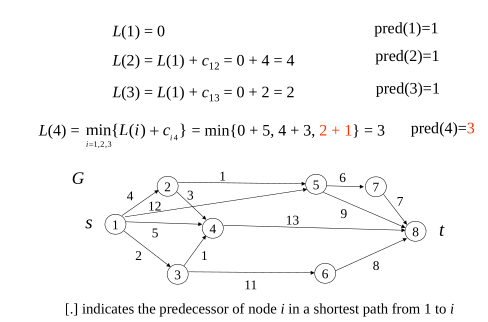
\includegraphics[width = \textwidth]{./images/DynProg.png}
					\end{figure}
					\begin{figure}[H]
						\centering
						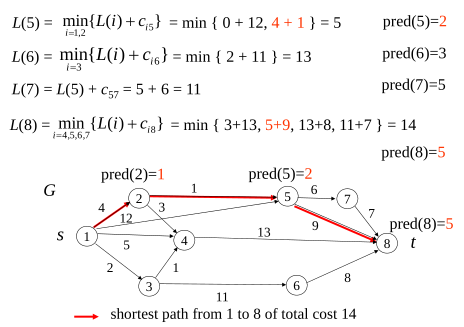
\includegraphics[width = \textwidth]{./images/DynProg2.png}
					\end{figure}


			\subsubsection{Project Planning}
				As shown in the Examples, we can use graphs to express dependency relationships. A direct application of this model is used when organizing various activitie inside a project: each phase will depend from some previous phases, there will be an "initial" phase with no predecessors and a final phase with no successors. The model adopted here is the one that represents
				\begin{itemize}
					\item \textit{activities} as arcs
					\item \textit{activity duration} with arcs weight
					\item \textit{checkpoints} as nodes
				\end{itemize}
				This formulation leads to a weighted directed acyclic graph. It's acyclic \textit{by nature}: it would be meaningless (and also logically incorrect) if activities in a project had circular relationships.\\
				This model helps in finding the \textit{minimum overall project duration}: being directed and acyclic, this will be the duration of the \textit{longest path} from the initial node to the final (we cannot compress the project time beyond that).

				\paragraph{Critical Path Method}
					The CPM aims to provide an optimal schedule for a project, with allotted time for each activity and the possible slack of each one, given the DAG of a project activities precedences. The algorithm is:
					\begin{enumerate}
						\item Construct the DAG of activities and precedences
						\item Topologically sorts the nodes
						\item For each node, calculate
							\begin{itemize}
								\item The earliest start time starting from inital activity. This would be (at the final node) the minimum overall project duration
								\item The latest time an activity can be started to NOT increase the minimum project duration (starting from the end, this time)
							\end{itemize}
						\item For each activity now we can calculate the \textit{slack}: $T_{max} - T_{min} - d$ where \emph{d} is the duration of the activity itself
					\end{enumerate}
					The slack of each activity indicates if it could be \textit{deliberately delayed} without affecting the overall project duration. There exist activities with null slack: these are called \underline{critical activities} and cannot be delayed in any case. They compose the critical path from the beginning to the end of the project.
			
			\subsubsection{Network Flows}
				Network flows problems are the ones that involves "distribution of a given resource over a network". Needless to say, they boils down to find the optimal throughput of a network given its \textit{Directed Weighted Graph} representation. In this kind of problems, we can remove the acyclicity hypothesis. The graph model we're dealing with is like:
				\begin{figure}[H]
					\centering
					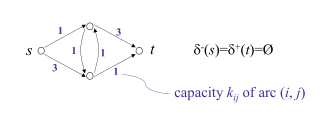
\includegraphics[width = \textwidth]{./images/Flows.png}
					\caption{Arcs weights assume a different meaning here: they are not more a cost or a lenght, but instead a \textit{width} or \textit{capacity} as shown in the blue note}
				\end{figure}
				We introduce the \textit{feasible flow vector}: it's a tuple of values representing the \textbf{occupated fraction} of each edge of the network; it should respects two major constraints:
				\begin{enumerate}
					\item Capacity constraints: $\forall (i, j) \in E\, |\, (0\, \leq\, x_{ij}\, \leq\, k_{ij} )$ where $x_{ij}$ is the value of the flow in the feasible flow vector, $k_{ij}$ the maximum capacity for that arc and \emph{E} the set of edges;
					\item Flow balance constraints: $\forall h \in N\, |\, (\sum(x_{ih}) = \sum(x_{hj}))$ that simply states that for each node, the amount that enters the node is the same amount that exits it
				\end{enumerate}
				We can then calculate the \textit{value of flow} $\phi = \sum(x_{sj})$, where \emph{s} is the initial node and j all the nodes reached by the \textit{outgoing cut} of \emph{s}; this represents the actual maximum flow that can go through the network.\footnote{The maximum flow is directly associated with the minimum capacity of a cut. Will see later how these, in fact, are mathematically correlated: \textit{they're dual problems}, or two representations of the same problem.}

				\paragraph{Ford Fulkerson's Algorithm}
					Another algorithm, this time to resolve a network flow problem. Again, this is just the algorithmic version of the intuitive solution for this problem: keep sending stuff on non-saturated channels until the network is maxed out.\\
					Said so, we need some additional definition to handle easily this algorithm:
					\begin{itemize}
						\item a \textit{backward arc} is an edge of the network that "sends units backward" with regard to a simil-topological ordering of the nodes. We can "flat out" the graph of the network to visually understand what a backward arc is:
							\begin{figure}[H]
								\centering
								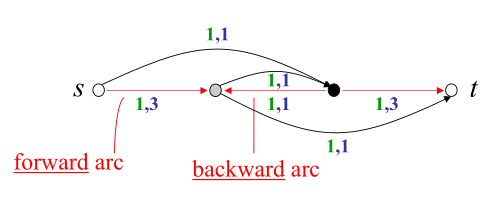
\includegraphics[width = \textwidth]{./images/BackwardArcs.png}
							\end{figure}
						\item an \textit{augmenting path} (wrt the current $\phi$) is a path through all the network (so start to end) where
							\begin{equation} 
								\begin{cases}
									x_{ij}\, <\, k_{ij} \text{ for all forward arcs}\\
									x_{ij}\, >\, 0 \text{ for all backward arcs}
								\end{cases}
							\end{equation}
						\item the \textit{residual network} of a graph is a graph itself buil keeping track of the possible changes that can be applied to the flows on the arcs. This means, if we have a \underline{saturated channel} with capacity 3 we will have in the residual network the same channel but \textit{reversed}: this signals that we have a residual capacity of 3 units \textit{in the opposite direction}.
							\begin{figure}[H]
								\centering
								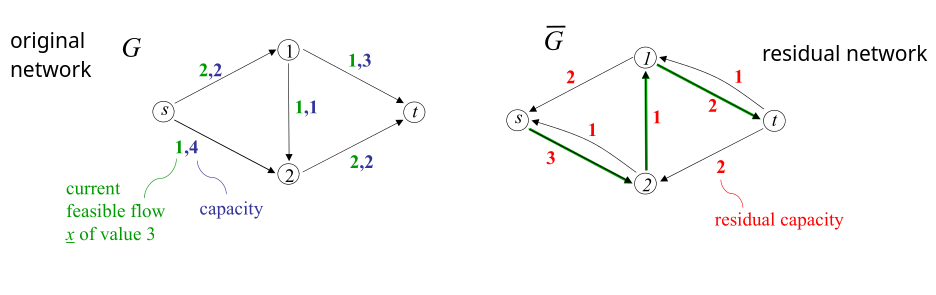
\includegraphics[width = \textwidth]{./images/Residual.png}
							\end{figure}
					\end{itemize}
					So, the algorithm is structured in 2 main phases:
					\begin{enumerate}
						\item Search for an augmenting path on the actual graph, then rebuild the residual graph. Repeat this point until no more trivial augmenting path can be found
						\item Look for an augmenting path \textit{on the residual graph}. Using the second graph is useful when some edges could be desaturated in order to maximize the flow. The algorithm stops when on the residual graph there are no more paths from \emph{s} to \emph{t}
					\end{enumerate}



	\clearpage
	\section{Complexity}
		An \textit{algorithm} is a set of instructions that allows a machine to solve all instances of a given problem. Its executions time depends on the instance itself (usually its dimension) and the computer carrying out the operations. The complexity of an algorithm is the "number  of elementary operations\footnote{memory access, arithmetic ops, conrontations} needed to complete it" in the worst case (so big-O scenario / notation).\\
		Complexity is used to estabilish two kind of things:
		\begin{itemize}
			\item The complexity of a given algorithm to solve a given problem
			\item The inherent difficulty of a problem
		\end{itemize}

		\subsection{Problems and Instances}
			If we want to estimate the performance of \textit{alternative} algorithm on a given problem, we should not forget that performances are conditioned by the instance size in a significative way. The formal definition for "size of an instance" is the number of bits needed to encode it. Quick example (take a look at indices)
			\begin{equation}
				I = \begin{cases}
					m\\
					c_1 ... c_m\\
				\end{cases}
			\end{equation}
			both $m$ and $c_j$ are integers. The computation of the instance size is:
			\begin{equation}
				\vert I \vert \,\leq\, \lceil \log_2(m) \rceil \,+\, m \,\times\, \lceil \log_2(c_{max}) \rceil
			\end{equation}
			Where $c_{max}$ is the maximum integer value among $c_j$. We take the max because we want to encode all numbers the same way. \textit{m is exactly the number of c values, pay attention}.

		\subsection{Complexity Classes}
			When looking at an algorithm we usually want to calculate its time complexity: we're looking for a function that is an upper bound of the time needed to complete, dependently from the instance size. This function is usually expressed with asymptotic terms, with the big-O notation. This said, we can divide algorithms in classes of complexity, wheter they are asymptotically similar. The two classes of complexity of interest are
			\begin{itemize}
				\item Polynomial: $O(n^d)$
				\item Exponential: $O(2^n)$
			\end{itemize}
			where $n$,as usual, indicates the instance size.

			\subsubsection{Complexity Classes for \emph{Problems}}
				We can identify the \textit{problems} with the algorithm\footnote{the most efficent so far, generally} that solves them. In this way, we can distinguish between "easy" and "hard" problems. We classify problems in the two infamous classes
				\begin{itemize}
					\item $\mathcal{P}$ problems: the recognition\footnote{estabilishing if a property is verified, a true/false response.} problems that can be \textit{solved in polynomial time}
					\item $\mathcal{NP}$ problems, or \textit{nondeterministic polynomial} problems; these problems CAN'T be solved in polynomial time\footnote{so far}, but a solution can be verified in polynomial time.
				\end{itemize}
				Speaking in Turing machine terms, the problems in class $\mathcal{P}$ can be solved by a standard Turing machine, while the ones in $\mathcal{NP}$ by a nondeterministic one. N.B.: the nondeterministic Turing machine is just a Turing machine that \textit{verifies}\footnote{in polynomial time} a \textit{guessed} solution, ence the name "nondeterministic polynomial".\\
				Millennium prize problem: is $\mathcal{P} \,\equiv\, \mathcal{NP}$?

				\paragraph{Reductions}
					Reducing a problem to another means, more or less, solving a problem with another one. We say that $P_1$ \textit{reduces in polynomial time} to $P_2$ if we can solve $P_1$ using an algorithm that solves $P_2$ as subroutine, calling it a \textit{polynomial number of times}.\\
					It's straightforward to notice that if the algorithm used to solve $P_2$ has constant complexity, then $P_1$ will have a overall polynomial complexity. A reduction where the second algorithm is called only once is a \textit{transformation}.

				\paragraph{$\mathcal{NP}$-complete problems}
					A problem is said to be $\mathcal{NP}$-complete $\Leftrightarrow$
					\begin{itemize}
						\item it belongs to $\mathcal{NP}$ and
						\item every other problem in $\mathcal{NP}$ can be reduced to it in polynomial time
					\end{itemize}
					So these problems are
					\begin{enumerate}
						\item nondeterministic polynomial, so hard to \underline{solve} but simple to \underline{verify} (hard means above-polynomial, simple means polynomial or less)
						\item complete, because we can use them to represents a whole set of problems
					\end{enumerate}
				
				\paragraph{$\mathcal{NP}$-hard problems}
					A problem is $\mathcal{NP}$-hard when "every other problem in $\mathcal{NP}$ can be reduced to it in polynomial time". This problematic definition is cleared by this observation, I think: all recognition problems that are $\mathcal{NP}$-complete have their optimization version that's $\mathcal{NP}$-hard. 

	\clearpage
	\section{Linear Programming}
		\subsection{Linear Programming Problems}
			A linear programming problem is an \textit{optimization} problem in the form
			\begin{equation}
				\begin{cases}
					\text{min } f(\underline{x})\\
					\text{s.t. } \underline{x} \in X \subseteq \mathbb{R}^n
				\end{cases}
			\end{equation}
			where
			\begin{itemize}
				\item $f: X \,\rightarrow\, \mathbb{R}$ is a \textit{linear function}
				\item the \textit{feasible region} $X \subseteq \mathbb{R}^n$ is a combination of linear functions.
			\end{itemize}
			We then define the \textit{optimal solution} of a linear programming problem as $\{\underline{\bar{x}}\, \vert\, f(\underline{\bar{x}}) \leq f(\underline{x})\}$ for all other vectors in the feasible region.\\
			LP problems can also be formulated with matrixes:
			\begin{equation}
				\begin{cases}
					\text{min } z = \underline{c}^t\, \underline{x}\\
					A\underline{x} \geq \underline{b}\\
					\underline{x} \geq \underline{0}
				\end{cases}
			\end{equation}

			\paragraph{Assumptions of LP Models}
				LP models and the algorithms operating on them work under several assumptions:
				\begin{enumerate}
					\item \underline{Linearity} of the objective function and constraints
					\item \underline{Divisibility} of the variables: there are no "undivisible units"
					\item \underline{Constant parameters} in the model. Also, accurate parameters
				\end{enumerate}

		\subsection{LP Problems Forms}
			The most general for for a linear programming model we can define is:
			\begin{equation}
				\begin{cases}
					\text{min/max } z = \underline{c}^t\, \underline{x}\\
					A_1\underline{x} \geq \underline{b_1}\\
					A_2\underline{x} \leq \underline{b_2}\\
					A_3\underline{x} = \underline{b_3}\\
					x_j \geq 0 \text{ for some \emph{j}}
				\end{cases}
			\end{equation}
			This form is usually referred to as \textit{canonical form}.

			\paragraph{Standard Form}
				The standard form is the "most restrictive" one, and also one of the easiest to work with
				\begin{equation}
					\begin{cases}
						\text{min } z = \underline{c}^t\, \underline{x}\\
						A\underline{x} = \underline{b}\\
						\underline{x} \geq \underline{0} 
					\end{cases}
				\end{equation}
				In this form, all constraints must be equalities, and all variables must be non negative. Pay attention: in the original general model, we have the non-negativity onstraints only on \underline{some} variables.

				\subparagraph{Transforming to Standard Form}
					We can easily transform a general formulation of a LP problem in standard one by applying these simple transformations:
					\begin{itemize}
						\item $\max(\underline{c}^t\underline{x}) = -\min(-\underline{c}^t\underline{x})$ to change objective function
						\item all inequalities are transformed adding a "slack variable":
							\begin{equation}
								\underline{a}^t\underline{x} \leq \underline{b} \Rightarrow
									\begin{cases}
										\underline{a}^t\underline{x} + s = \underline{b}\\
										s \geq 0
									\end{cases}
							\end{equation}
							or a surplus variable in case it's a $\geq$ inequality
							\begin{equation}
								\underline{a}^t\underline{x} \geq \underline{b} \Rightarrow
									\begin{cases}
										\underline{a}^t\underline{x} - s = \underline{b}\\
										s \geq 0
									\end{cases}
							\end{equation}
						\item when a variable is unrestricted in sign it's "splitted" in its positive and negative part:
							\begin{equation}
								x_j \in \mathbb{R} \Rightarrow
									\begin{cases}
											x_j = x_j'-x_j''\\
											x_j' \geq 0\\
											x_j'' \geq 0
									\end{cases}
							\end{equation}
					\end{itemize}

		\subsection{Geometry of a LP Problem}
			We assume known the notions of "level curve" for a function (a set of points where a multi variable function is constant) and gradient\footnote{Also its geometric interpretation as the \textit{direction of maximum growth}.}.

			\subsubsection{Feasible Region as an Hyperplane}
				By definition, $\{x \in \mathbb{R}^n \,\vert\, \underline{a}^tx = \underline{b}\}$ is an hyperplane, while $\{x \in \mathbb{R}^n \,\vert\, \underline{a}^tx \geq \underline{b}\}$ an affine half space, defined as a combination of all inequality constraints.\\
				So, the \textit{feasible region} of an LP problem, defined as \textit{a region delimited by hyperplanes}, is called a \textit{polyhedron}. A polyhedron (so a polygon in two dimension, a 3D figure in three dimension and so on) is a \underline{convex} set of $\mathbb{R}$ as generated by convex sets.
				\begin{figure}[H]
					\centering
					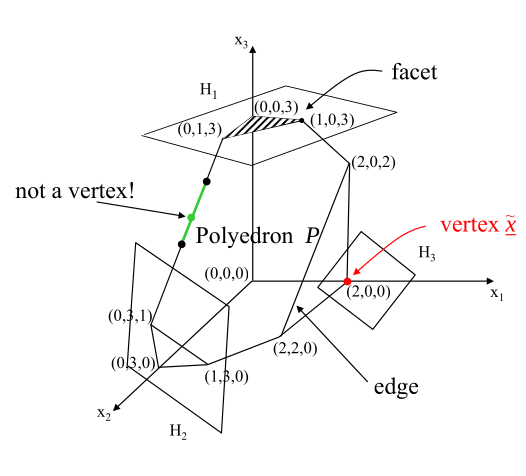
\includegraphics{./images/Polyhedron1.png} %% perfect image size woah
				\end{figure}
				We call a \textit{convex combination} a linear combination where all coefficients are non negative and sum to 1. We define a \textit{vertex} of a polyhedron as a point in the ph that cannot be expressed as the convex combination of two other dintinct points in the ph. Don't worry if you're confused: all "polyhedra theory" has a lot of dark spots\footnote{check out they wikipedia page}. Non-empty polyhedra representing an LP problem (in both canonical or standard form) \textbf{has a finite number of vertices}, greater or equal to one\footnote{a polyhedron with only one vertex is a quarter of plane, for example}.\\
				We can represent \textit{every point of a polyhedron} as a convex combination of its \textit{vertices} plus (if needed) a vector that never ends inside the polyhedron (for unbounded polyhedron).
				\begin{figure}[H]
					\centering
					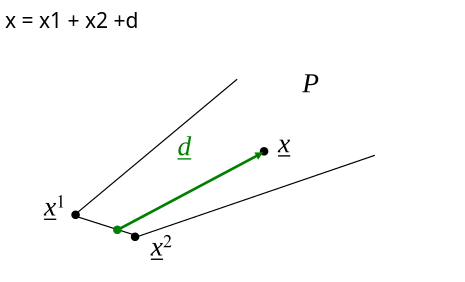
\includegraphics{./images/Polyhedron2.png}
					\caption{Every point of this unbounded polyhedron can be represented as a combination of $x_1$ and $x_2$ and $\underline{d}$, where $\underline{d}$ is called \textit{unbounded feasible direction} of the polyhedron.} 
				\end{figure}

				\subsubsection{Fundamental Theorem of Linear Programming}
					Consider a LP $\{\min(\underline{c}^tx\}$ where $x \in P$, which is a non-empty polyhedron of the feasible solutions (in standard or canonical form). Then either
					\begin{enumerate}
						\item exists at least a single optimal vertex
						\item the value of the objective function is unbounded below on $P$
					\end{enumerate}
					This foggy theorem has a simple intuitive interpretation, in my mind: the feasible region is represent as a subset of $\mathbb{R}$ and reprents \textit{all the solutions of the system of constraints}. To minimize the objective function, we must "move around" this subspace in a well-defined direction, that is the opposite of the gradient of the objective function itself. Being this a \textit{straight line}, we will eventually hit a boundary of the polyhedron. We could then "slide" onto it until we are "stuck" and every move we make is not anymore bettering the solution. This can happen \textit{only} on the intersection of boundaries (so the vertices), because it's the only point where a "direction" to better the solution finds his boundary\footnote{I find this mumbo jumbo more clear than the slides definition, ok? In my head it's clear this way.}.\\
					This theorem allows us to do determine a priori which are our solutions, just looking at the way the feasible region is defined. Also, being \textit{finite}, we can cycle through the solutions to "easily" find the right one.

		\subsection{Algebraic Characterization of the LP Problem}
			We've seen we can exploit the geometry of the feasible region to find the solutions. We need an algebraic formulation to do that algorithmically.

			\subsubsection{The Feasible Vector Space}
				Classic LP problem: $P=\{x \in \mathbb{R} \,\vert\, Ax = b, x \geq \underline{0}\}$ in standard form. We assume from now on that $A$ is full rank. This leads to two possible scenarios:
				\begin{itemize}
					\item $A$ is a square matrix $\Rightarrow$ there exists only a \textit{unique} solution to the system: $x = A^{-1}b$.
					\item $A$ is a rectangular matrix with more columns than rows: this leads to infinite solutions of the system.
				\end{itemize}
				Obviously, having the exact number of constraints equal to the variables one is not common. We focus on the second case.\\
				If we partition the matrix $A = [B \,\vert\, N]$, where $B$ is a basis\footnote{set of linearly indipendent vectors} and $N$ the "remaining" vectors, we can redefine the solutions' vector as:
				\begin{equation}
					x = (x_B,\, x_N)
				\end{equation}
				where the two components of the vector will be long as the rank of the matrix and the lenght of the remaining matrix. We then substitute into the feasible region definition
				\begin{equation}
					Bx_{B} + Nx_{N} = \underline{b}
				\end{equation}
				and so
				\begin{equation}
					x_{B} = B^{-1}\underline{b} - B^{-1}Nx_{N}
				\end{equation}
				from this last equation, we can define
				\begin{itemize}
					\item a \underline{basic solution} is a solution setting all non base variables $x_{N}$ to zero, so $x_B = B^{-1}\underline{b}$
					\item a \underline{basic \textit{feasible} solution} is a basic solution that has all components greater or equal to zero
					\item the variable in $x_B$ are called \underline{basic variables} and the ones in $x_N$ \underline{non basic variables}
				\end{itemize}
				Now we link the algebraic formulation with the geometrical interpretation:

				\paragraph{Theorem}
					$x \in \mathbb{R}^n$ is a \textit{basic feasible solution} $\Leftrightarrow$ $x$ is a \textit{vertex} of $P = \{x \in \mathbb{R}^n \,\vert\, Ax = \underline{b}, x \geq \underline{0}\}$

		\subsection{The Simplex Method}
			Dantzig's simplex method is an algorithm to find the best basic feasible solution of a LP problem: it examines a sequence of BFSs with \textit{non increasing objective function values} until an optimal solution is reached, or the problem is found to be \textit{unbounded}.

			\subsubsection{The Algorithm}
				\begin{enumerate}
					\item check for infeasibility of the problem
					\item find an initial vertex
					\item move from a current vertex to a \textit{better adjacent vertex} (or estabilish that the problem is unbounded)
					\item determine if the current vertex is \textit{optimal}
				\end{enumerate}

				\paragraph{Infeasibility Check}
				To check if a problem is infeasible, we create an auxiliary problem with artificial variables (from the original problem) as:
					\begin{equation}
						P = 
						\begin{cases}
							\min z = \underline{c}^t x\\
							Ax = \underline{b}
							x \geq \underline{0}
						\end{cases}
					\end{equation}
					\begin{equation}
						P_{aux} = 
						\begin{cases}
							\min v = \sum_{i = 1}^m y_i\\
							Ax + Iy= \underline{b}\\
							x \geq \underline{0}, y \geq \underline{0}
						\end{cases}
					\end{equation}
					obviously, there exists a BFS composed by all elements in \emph{y}. We face two cases now:
					\begin{enumerate}
						\item $v > 0$ the problem is \textit{\textbf{infeasible}}
						\item if $v = 0$, the problem is feasible and we must manipulate the matrix in order to obtain a BFS that only depends on the original $x_i$ variables
					\end{enumerate}
					Don't forget we have to turn to the original problem and recompute the objective function.

				\paragraph{Initial Vertex Selection}
					The selection of a starting initial BFS is a problem per se. If the problem is easy enough we'll have the initial matrix already in a $A = [N \,\vert\, I]$ form, where \emph{I} represents the identity matrix $\Rightarrow$ a basic feasible solution. In that case, we have already a perfect indication of which variables are in the basis and at which cost, so we can directly go to the "movement" phase (that's the one that really optimizes the objective function value).\\
					In the other case (that's obviously more realistic) we have to resort again at the "auxiliary problem" with artificial variables: the initial basis we find is the one determined by the $y_i$ vectors.

				\paragraph{Movement Across Vertices}
					To "move" from a vertex to another means to swap some of the basic vertices out of the solution and "bring in" some of the vectors that were in the $N$ matrix. \textit{Algebrically}, this means to \textit{expressing the basic variables in terms of the non basic ones}. \textbf{Remember}: non basic variables are set to \textbf{zero}. Algorithmically, this is done through a simple pivoting operation on the combined $[B\vert N]b$ matrix.\\
					Given $Ax = \underline{b}$
					\begin{enumerate}
						\item select a coefficient $a_{rs} \neq 0$ of table $A$ where \emph{r} is the row index and \emph{s} is the column index
						\item divide row \emph{r} for $a_{rs}$ (also in order to have $a_{rs} = 1$)
						\item for alla other rows, subtract row \emph{r} multiplied by the coefficient on column \emph{s}: that is, $a_{is}$
					\end{enumerate}
					This will render the \emph{s} column all zeroes except the 1 on row \emph{r}. Don't forget we're applying this procedure also the the $\underline{b}$ vector.
					\begin{figure}[H]
						\centering
						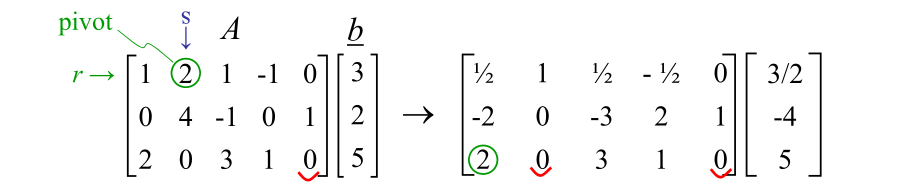
\includegraphics[width = \textwidth]{./images/Simplex1.png}
					\end{figure}
					The choice of \emph{r} and \emph{s} are crucial: in fact, they select which variable enters the basis (through the pivot column) and which leaves it (through the pivot row). This choice can be taken
					\begin{itemize}
						\item randomly
						\item using heuristics
						\item usign \textbf{Bland's rule}, that also avoid cycles in the algorithm
					\end{itemize}

					\subparagraph{Bland's Rule}
						Bland's rule dictate a choice for rows and columns to enter/leave the basis. It states:
						\begin{enumerate}
							\item select \emph{s} the \textit{first column with negative reduced cost}
							\item then select \emph{r} the row with the \textit{smallest} $\frac{b_r}{a_{rs}}$ ratio \textbf{among the positive ones}
						\end{enumerate}
						This simple criterion avoids cycles in the Simplex algorithm, that can be stuck in a vertex for some degenerate LP problems. In practice, due to the additional complexity added and the rarity of such problems, Bland's rule is never used.

					\subparagraph{Tableau Representation}
						As spoiled when talking about movement across vertices, the Simplex method has a peculiar way to represent the matrixes and vectors it uses to ease the computing problem.\\
						Given
						\begin{equation}
							P = 
							\begin{cases}
								z=\underline{c}^t x\\
								Ax = \underline{b}
							\end{cases}
						\end{equation}
						We initialize the tableau of values as
						\begin{figure}[H]
							\centering
							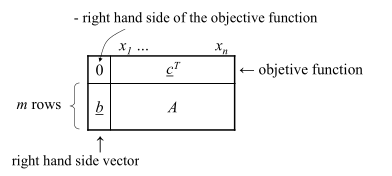
\includegraphics[width = \textwidth]{./images/Simplex2.png}
						\end{figure}
						Then we proceed (through the pivoting operation) to put the tableau in canonical form:
						\begin{figure}[H]
							\centering
							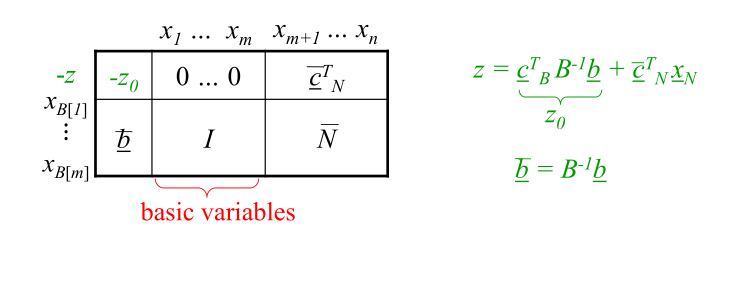
\includegraphics[width = \textwidth]{./images/Simplex3.png}
						\end{figure}


				\paragraph{Optimality Check}
					To check if a solution is optimal we cannot only watch the feasible region, we must take into account also the objective function. We repeat the reasoning made for finding the expressions of BFSs: given $x_B = B^{-1}\underline{b} - B^{-1}N\underline{x_N}$ basic solution and posing $x_N$ equal to zero to find the basic feasible solution, we can express the $\{\min(\underline{c}^tx)\}$ objective function as
					\begin{equation}
						\underline{c}^tx = (c_B, c_N) * \begin{pmatrix} x_B \\ x_N \end{pmatrix} = 
							\begin{pmatrix}
								B^{-1}\underline{b} - B^{-1}N\underline{x_N} \\
								x_N
							\end{pmatrix}
					\end{equation}
					we can now separate
					\begin{equation}
						\underline{c}^tx = \underbrace{c_B^tB^{-1}b}_{z_0} + \underbrace{(c_N^t - c_B^tB^{-1}N)x_N}_{\underline{\overline{c_N}}}
					\end{equation}
					where
					\begin{itemize}
						\item $z_0$ is a \textit{constant value} and is called cost of the basic feasible solution
						\item the second term $\underline{\overline{c_N}}$ is a function \textit{only of the non basic variables} and is the \textit{reduced cost} o the non basic variables
					\end{itemize}
					We can also define de vector of reduced costs wrt the basis itself: $\underline{\overline{c}} = \underline{c}^t -\underline{c}_B^tB^{-1}A$ that is
					\begin{equation}
						\begin{pmatrix}
							c_B^t - c_B^tB^{-1}B \\
							c_N^t - c_B^tB^{-1}N
						\end{pmatrix}
						=
						\begin{pmatrix}
							0 \\
							\underline{\overline{c_N}}
						\end{pmatrix}
					\end{equation}
					The reduced costs gives a measure on how much the objective function changes wrt a change in the value of the variable. Also, they provide a sufficent (but not usually necessary) condition for \textbf{optimality}: if all reduced costs of non basic variables are non negative, then the basic feasible solution associated to that non negative variables is optimal. So, more formally:\\
					Given $P = \{\underline{c}^tx : [B \vert N]x = \underline{b}, x \geq \underline{0}\}$
					\begin{equation}
						\underline{\overline{c_N}} \geq \underline{0} \Rightarrow (x_B, x_N) \text{ s.t. } x_B = B^{-1}\underline{b} \geq \underline{0} \,\wedge\, x_N = \underline{0}, x_B \text{ is optimal}
					\end{equation}

		\subsection{Duality}
			The \textbf{duality} concept for linear programming can be explained as: to any minimization (maximization) LP problem we can associate a closely related maximization (minimization) LP problem \textit{based on the same parameters}. For example, the famous maximum network flow problem is the dual of the minimum capacity cut problem.

			\subsubsection{Building the Dual Problem}
				Given a maximization problem $P = \{\max \underline{c}^tx, Ax \leq \underline{b}\}$ any feasible solution provides a \textit{lower bound} of the objective function value. "Which one is the best lower bound"? Can we "flip" the problem to a minimization one?\\
				The basic idea is to find a \textit{linear combination of the constraints} in such a way that the obtained value for the constraints \textit{dominates}\footnote{has a higher value} the objective function. So, a new set of variables should be introduced (the coefficents of the linear combination) and should be linked to the \textit{coefficents of the objective value}. These new constraints will create the new feasible region. The objective function the must be changed also: it has to tune each new constraint with the original value of such equation. An example will do the trick.

				\paragraph{Example}
					Given
					\begin{equation}
						\begin{cases}
							\max z = 4x_1+x_2+5x_3+3x_4 \\
							\begin{pmatrix}
								1 & -1 & -1 & 3 \\
								5 & 1 & 3 & 8 \\
								-1 & 2 & 3 & -5
							\end{pmatrix}
							\times
							\begin{pmatrix}x_1 \\ x_2 \\ x_3 \\ x_4\end{pmatrix}
							\leq
							\begin{pmatrix}1 \\ 55 \\ 3\end{pmatrix} \\
							x \geq \underline{0} 
						\end{cases}
					\end{equation}
					If we just multiply the second row of matrix \emph{A} for $\frac{5}{3}$, we obtain a disequality that dominates the objective function. We also obtain such a constraint if we add the second and the third row of the matrix. This two operations generate a \textit{valid constraint} that also \textit{brings information about the objective function}: it gives the obj an upper bound.\\
					Generalizing this reasoning, we can define a linear combination of the constraints, and also linarly combine them with the right hand side vector \emph{b}, to have actually a whole new set of constraints that is also consistent
					\begin{equation}
						y_1 * (\text{ first line of A }) + y_2 * (\text{ second line of A }) + y_3 * (\text{ third line of A }) \leq y_1 + 55y_2 + 3y_3
					\end{equation}
					Now we can factorize the above equation in order to isolate the $x_i$ variables. Then, we turn back to imposing that the \textit{coefficient for $x_i$ must be greater or equal to the one of the objective function} in order to dominate it.
					\begin{equation}
						\begin{pmatrix}
							1 & 5 & -1 \\
							-1 & 1 & 2 \\
							-1 & 3 & 3 \\
							3 & 8 & -5 \\
						\end{pmatrix}
						\times
						\begin{pmatrix}y_1 \\ y_2 \\ y_3\end{pmatrix}
						\geq
						\begin{pmatrix} 4 \\ 1 \\ 5 \\ 3 \end{pmatrix}
					\end{equation}
					we can see as the last vector is just the $\underline{c}$ vector of the original problem. Given that we're now looking for an upper bound of \emph{z}, and also the \textit{lowest} upper bound, the dual problem will be a minimization problem; also, every "constraint coefficient" variable will contribute to the objective function proportionally to their right hand side coefficient of the original problem. We can now formulate the full dual problem:
					\begin{equation}
						\begin{cases}
							\min v = y_1 + 55 y_2 + 3 y_3 \\
							\begin{pmatrix}
								1 & 5 & -1 \\
								-1 & 1 & 2 \\
								-1 & 3 & 3 \\
								3 & 8 & -5 \\
							\end{pmatrix}
							\times
							\begin{pmatrix}y_1 \\ y_2 \\ y_3\end{pmatrix}
							\geq
							\begin{pmatrix} 4 \\ 1 \\ 5 \\ 3 \end{pmatrix} \\
							y \geq \underline{0}
						\end{cases}
					\end{equation}

			\subsubsection{General Form of the Dual Problem}
				As could be derived from the example, the relation between th \textbf{primal} and \textbf{dual} problem is
				\begin{equation}
					(P) = 
					\begin{cases}
						\max z = \underline{c}^tx \\
						Ax \leq \underline{b} \\
						x \geq \underline{0}
					\end{cases}
				\end{equation}
				\begin{equation}
					(D) = 
					\begin{cases}
						\min v = \underline{b}^ty \\
						A^ty \geq \underline{c} \\
						y \geq \underline{0}
					\end{cases}
				\end{equation}
				The duality relation is symmetric: if \emph{D} is the dual of \emph{P}, then the dual of \emph{D} is \emph{P}.\\
				When dealing with problems in standard form, the non negativity constraint on the vector $y$ is not more needed.\\
				Another formulation for this problem that keeps into account the basic and nonbasic solutions is:
				\begin{multicols}{2}
					\begin{equation}
						(P) = 
						\begin{cases}
							\min z = c_Bx_B + c_Nx_N \\
							Bx_b + Nx_N = b \\
							x_B,\, x_N \geq \underline{0}
						\end{cases}
					\end{equation}
					\break
					\begin{equation}
						(D) = 
						\begin{cases}
							\max v = yb \\
							yB \leq c_B \\
							yN \leq c_N
						\end{cases}
					\end{equation}
				\end{multicols}

			\subsubsection{Weak Duality Theorem}
				Given the classical formulation for a linear programming problem and its dual:
				\begin{multicols}{2}
					\begin{equation}
						(P) = 
						\begin{cases}
							\max z = \underline{c}^tx \\
							Ax \leq \underline{b} \\
							x \geq \underline{0}
						\end{cases}
					\end{equation}
					\break
					\begin{equation}
						(D) = 
						\begin{cases}
							\min v = \underline{b}^ty \\
							A^ty \geq \underline{c} \\
							y \geq \underline{0}
						\end{cases}
					\end{equation}
				\end{multicols}
				the \textit{weak duality theorem} states that for every feasible solution $\underline{\overline{x}} \in X$ of $(P)$ and every feasible solution $\underline{\overline{y}} \in Y$ of $(D)$ we have
				\begin{equation}
					\underline{b}^t\underline{\overline{y}} \leq \underline{c}^t\underline{\overline{x}}
				\end{equation}
				This is easy to visualize if we imagine the two problems (and in particular, the two feasible regions) as opposite but with the same objective: one is trying to reach the optimal solution by increasing the objective function value, the other doing the opposite reducing it. This leads us to the next important property of dual problems:

			\subsubsection{Strong Duality Theorem}
				Given primal and dual problem as in (31) and (32), and given that they are both \textit{bounded} and \textit{feasible}, then if $x^*$ is an optimal solution for $(P)$ and $y^*$ is an optimal solution for $(D)$ we have that
				\begin{equation} \underline{c}^tx^* = \underline{b}^ty^* \end{equation}
				\begin{minipage}{0.5\linewidth}
					Again, this is just an extension of what we've said for the weak duality theorem: the visualization is also very simple, as shown in the figure
				\end{minipage}
				\begin{minipage}{0.5\linewidth}
					\begin{figure}[H]
						\centering
						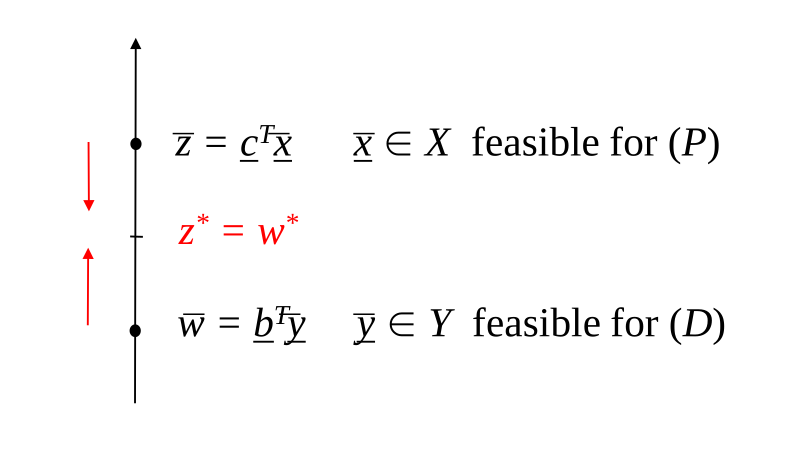
\includegraphics[width = \textwidth]{./images/Duality1.png}
						\caption{Relation between feasible regions and optimal solutions of dual problems.}
					\end{figure}
				\end{minipage}
				\vspace{0.5cm}
				
				in the end, we have 4 possible cases out of 9 possible combination of problems, that are explained in the table below:
				\begin{center}
					\begin{tabular}{ m{2.5cm} || m{4cm} | m{4cm} | m{4cm} | }
						& $\exists$ an optimal solution & unbounded problem & infeasible problem \\
						\hline
						\hline
						$\exists$ an optimal solution & Granted by the strong duality theorem & Not possible (SDT) & Not possible (SDT) \\
						\hline
						unbounded problem &  & not possible (WDT) & consequnce of weak duality theorem \\
						\hline
						infeasible problem &  &  & only possible combination for empty feasible region\\
						\hline
					\end{tabular}
				\end{center}
				where obviously columns and rows represent the possible condition of the primal and dual problem. As said, the relation is symmetric (so only half of the matrix is shown) and SDT and WDT means Strong Duality Theorem and Weak Duality Theorem.

			\subsubsection{Optimality Conditions}
				The strong duality theorem gives us a powerful tool to prove the optimality of a solution of the linear problem: if we find $x^*$ optimal solution for the primal problem and $y^*$ optimal solution for the dual, it must hold that $\underline{c}^tx^* = \underline{b}^ty^*$. This can be easily proven by substituting the definition of the vectors inside the equation given:
				\begin{equation}
					\begin{cases}
						Ax^* = \underline{b} \\
						A^ty^* = \underline{c} \\
						\Rightarrow \,\, y^{*t} \underline{b} = y^{*t}Ax^* = \underline{c}^tx^*
					\end{cases}
				\end{equation}

			\subsubsection{Complementary Slackness}
			Following along the reasoning that gaves us the new Optimality Conditions, we can see a lso a relation between \textit{slack variables} of optimal solution. Let's say $x^* \in X \text{ and } y^* \in Y$ optimal solutions for the primal and the dual problem respectively. We can notice that
			\begin{equation}
				\begin{cases}
					\forall i \,\vert\, y_i^*(a_i^tx^*-\underline{b}_i) = 0 \\
					\forall j \,\vert\, (\underline{c}_i^t - y^{*t}a_j)x_j^* = 0
				\end{cases}
			\end{equation}
			Where \emph{i} and \emph{j} represents respectively the row index and the column index of the \emph{A} table. We can see that at \textit{optimality}, the product of each variable with the corresponding slack variable of the constraint of the relative dual is null. This \textit{again} gives us a way to easily detect optimality in a solution and to find the dual one: it's enough to check the complementary slackness equations once found a solution.

		\subsection{Sensitivity Analisys}
			"How much does an optimal solution change wrt the variations of some of its parameters?"\\
			This is sensitivity analysis, so calculate and quantify the effect produced on the optimal objective function value by a variation in the parameter value. This is useful when adjustments must be made, and we have to choose which parameter ensures the maximum or minimum variation overall. Remember: in sensitivity analysis \textit{everything} is a parameter, from the optimal solution values to the right hand side vector of the feasible region definition.

			\subsubsection{Optimality Intervals}
				A direct application of sensitivity analysis is to find the interval in which a basis \emph{B} remains optimal\footnote{so that $B^{-1}\underline{b}$ remains non negative with $x_N$ set to zero, and th reduced costs of the variables in the basis remain non negative too.}. In this case, we can vary the cost coefficents and the right hand side termns in order to verify the intervl of validity of a base.

				\paragraph{Tweaking the \emph{\underline{b}} Vector}
					We have the optimal solution $\underline{x}^* = \begin{pmatrix} B^{-1}(\underline{b}) \\ \underline{0} \end{pmatrix}$, we modify \emph{slightly} the solutions vector, we obtain:
					\begin{equation}
						x^* = 
						\begin{pmatrix}
							B^{-1} ( \underline{b}\, +\, \delta \underline{e} ) \\
							\underline{0}
						\end{pmatrix}
					\end{equation}
					where as usual the nullifiedpart of the vector is the one associated to the non basic variables, and \emph{e} represents a column of the identity matrix. In systesys, we're modifyin just a single entry of the solutions vector, by $\delta$. We just apply the definition of optimality for a basis and have that \textit{B remains optimal as long as}
					\begin{equation}
						B^{-1} ( \underline{b}\, +\, \delta \underline{e} ) \geq \underline{0} \,\Rightarrow\, B^{-1}\underline{b} \geq -\delta B^{-1} \underline{e}
					\end{equation}
					Obviously, changing the value of the basic vectors impacts the value of the objective function, which goes from $\{\underline{c}^tB^{-1}\underline{b}\}$ to $\{ \underline{c}^tB^{-1} ( \underline{b}\, +\, \delta \underline{e} ) \}$.

				\paragraph{Tweaking the \emph{\underline{c}} Vector}
					We increment just as before the cost coefficient vector as $\underline{c}' = \underline{c}\, +\, \delta \underline{e}$. The basis remains optimal as long as
					\begin{equation}
						\underline{c}_N^{'t}\, -\, \underline{c}_B^{'t}B^{-1}N \geq \underline{0}
					\end{equation}
					In this case, we're changing the objective function value, but \textit{differently from the previous case} the $x^*$ vector remain unchanged.
	
	\clearpage
	\section{Integer Linear Programming}
		An ILP problem is a Linear Programming problem with the additional constraint $\underline{x} \in \mathbb{Z}^n$. Obiously we could add the integer constraints only to some varibales: in that case, the problem is said \textit{mixed} integer LP. An assumption we make (that does not influence the reasoning or the outcome) is that both \emph{A} and \emph{\underline{b}} are also composed of integers values.

		\subsection{Linear Relaxation and Relation with Linear Programming}
			If we remove the integer constraint froman ILP problem, weare left with a simple linear problem that shares some properties with the starting integer one:
			\begin{multicols}{2}
				\begin{equation}
					ILP: 
					\begin{cases}
						\max \underline{c}^tx \\
						Ax \leq \underline{b} \\
						x \geq \underline{0} \\
						x \in \mathbb{Z}^n
					\end{cases}
				\end{equation}	
				\break
				\begin{equation}
					LP:
					\begin{cases}
						\max \underline{c}^tx \\
						Ax \leq \underline{b} \\
						x \geq \underline{0}
					\end{cases}
				\end{equation}
			\end{multicols}
			The second one is called \textit{linear continuous relaxation} of the integer problem. For each ILP problem, we have that
			\begin{itemize}
				\item The objective function value of the optimal solution of the integer problem is always \textit{smaller in module} wrt the one of the linear relaxation
				\item The feasible region of the ILP problem is fully contained inside the one of the continuous relaxation: $X_{ILP} \subseteq X_{LP}$
			\end{itemize}
			\begin{minipage}{0.5\linewidth}
				These two properties are easily explained by the graphical representation of the feasible regions: it's easy to see how the "discreteness" of the ILP problem produces a "loss" of information (as the fractional part of solutions) and thus "reduces" the dimension of the feasible region.
			\end{minipage}
			\begin{minipage}{0.5\linewidth}
				\begin{figure}[H]
					\centering
					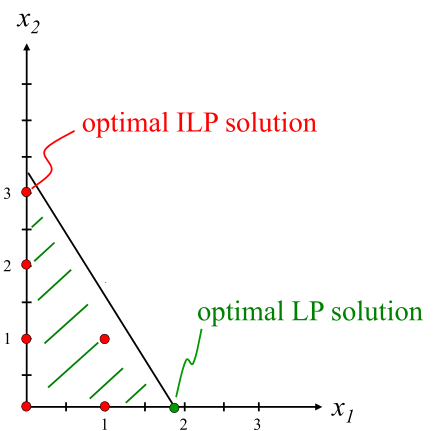
\includegraphics[width = \textwidth]{./images/ILP1.png}
				\end{figure}
			\end{minipage}

		\subsection{Solving an ILP Problem}
			The first naive approach to solve an ILP problem could be to find the solutions of the associated linear relaxation, the round them to the "nearest" integer value that respects the boundaries. This method is not perfect because often the rounded solutions are \textit{infeasible} for the ILP problem or even \textit{useless}. The best application of this approach is when the objective function value is optimal for "large" numbers, so rounding does not affect in a significative way the actual OFV.\\
			Instead of focusing on the linear relaxation, we can directly solve the ILP problem exploiting its peculiarities:
			\begin{itemize}
				\item Implicit enumeration techniques explore all the feasible solutions by "traversing" them. In this category fall the "branch and bound" method but also dynamic programming techniques
				\item Cutting planes strategy aims to exploit the geometry of an integer problem, tuning the constraints of the feasible region in order to achieve an integer-bound feasible region to isolate easily a solution
				\item all sorts of heuristics can be used. These are not exact methods thogh.
			\end{itemize}

			\subsubsection{Branch and Bound Method}
				The idea behind branch and bound method is the classic "divide et impera" approach in algorithm design. In this particular problem, "divide" becomes "partition the feasible region into subregions" and "impera" is "resolve the problem locally in the subregion".

				\paragraph{Branching}
					Given the classic minimization problem $\{\min(c(x)) \,\vert\, x \in X\}$ we partition the feasible region as $X = \bigcup X_n$ with $X_i \bigcap X_j = \emptyset,\, i \neq j$. We can define $z_i = \min(c(x)) \,\vert\, x \in X_i$, so to have that the \textit{global} minimum is the minimum among all these \textit{local} $z_i$ minima. In an ILP problem, partitioning is really straightforward: we initially find a candidate solution for the linear relaxation: if such solution $\underline{x}$ is fractional, we divide the problem in the "greater or equal then" and "less or equal then" the integer approximation of the solution $\underline{x}$

				\paragraph{Bounding}
					For each subproblem defined by the branching phase, we can do three things:
					\begin{itemize}
						\item prove that the selected subregion of $X$ is empty
						\item prove that the objective function value won't decrease if we search in this subregion (so skipping the analysis for this particular subregion)
						\item determine a local optimal solution and update the value of the objective function found so far
					\end{itemize}
					this is a recursive method: we can also branch subregions and repeat the reasoning inside these subsubregions and so on.\\
					In an ILP, we just look for the solution of the linear relaxation of each subregion.

				\paragraph{B\&B Algorithm Summary}
					\begin{enumerate}
						\item Find the solution of the linear relaxation of the ILP considered
							\begin{itemize}
								\item if the solution is integer, return this value
								\item if it's fractional, go to step 2
							\end{itemize}
						\item $x_{LR}$ the solution at step 1, divide the feasible region in $x \leq \lfloor x_{LR} \rfloor$ and $x \geq \lfloor x_{LR} \rfloor + 1$ and return at step 1
					\end{enumerate}
					\begin{minipage}{0.5\linewidth}
						\begin{figure}[H]
							\centering
							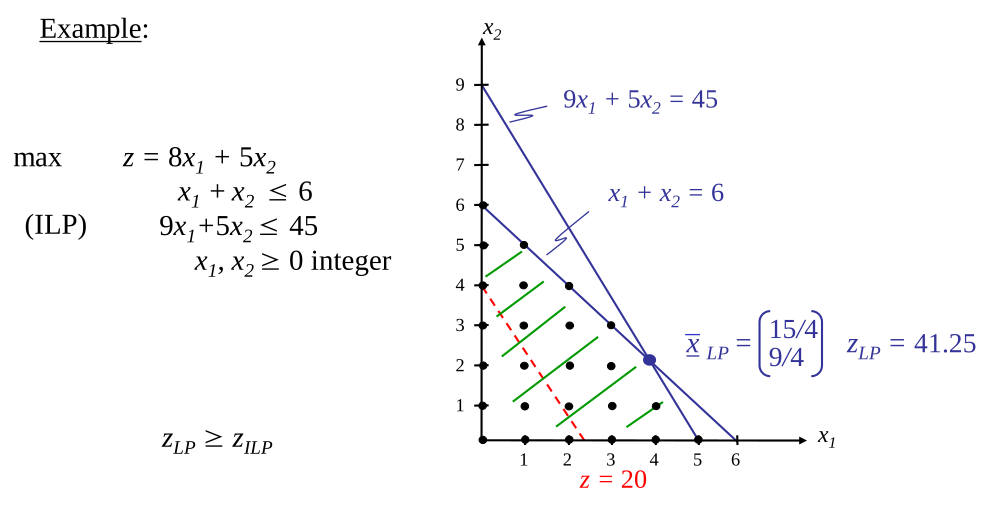
\includegraphics[width = \textwidth]{./images/BaB1.png}
							\caption{The problem}
						\end{figure}
					\end{minipage}
					\begin{minipage}{0.5\linewidth}
						\begin{figure}[H]
							\centering
							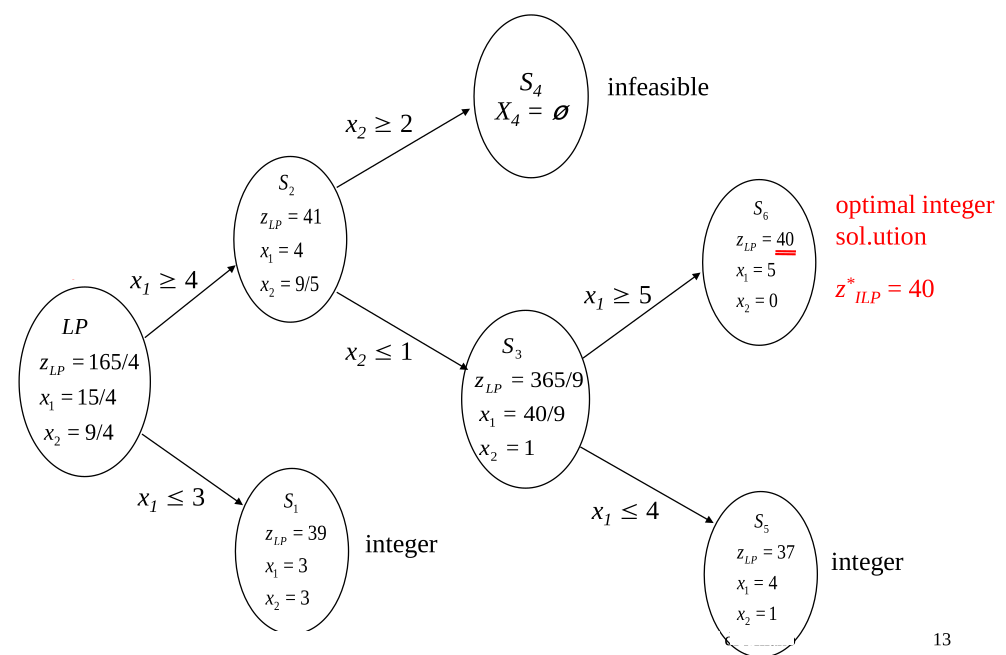
\includegraphics[width = \textwidth]{./images/BaB2.png}
							\caption{Branch and bound decision tree with local solution values}
						\end{figure}
					\end{minipage}
					\vspace{0.5cm}
					
					The choice of "which subnode to evaluate next" can be done following the "deeper path" (so trying to fix the major number of nodes sequentially, the simplest version of the algorithm) or following the most promising nodes (the greedy approach). 

			\subsubsection{Cutting Plane Method and Gomory Fractional Cut}
				The B\&B method is a good method to find integer solutions of an ILP problems, but has the common problem of recursive tree-based algorithms: overall temporal complexity, difficult to evaluate single nodes etc. The cutting planes method aims, as already said, to exploit the peculiarity of the "integer geometry" of the ILP feasible region.\\
				The idea is: the polyhedron described by the feasible region could be "readjusted" in order to costraint \textit{exactly} the integer solutions, and not also the fractional part of the relaxation. It's easily explained by an example: if the "rightmost" constraint of our two-dimensional feasible region is $x \leq 2.15$, we can readjust the constrainf to $x \leq 2$ without losing solutions of the ILP problem. Also, it would be simpler to find an exact optimal solution along this constraint. If we repeat the reasoning for all rows of matrix $A$, we could "shrink" the feasible region down to have just the integer solutions on the vertices. We define an \textit{ideal formulation} of the feasible region as the one that describes the \textit{convex hull} of $X_{ILP}$, so the \textit{smallest convex set that encloses} $X_{ILP}$. REMEMBER: $X_{ILP}$ is a \underline{discrete} set, while the hull is a continuous polyhedra. This definition is useful when paired when the theorem:\\
				for any feasible region $X_{ILP}$ of an integer linear programming problem, there exists an ideal formulation involving a finite number of linear constraints.\\
				Usually, the number of constraints of the ideal formulation is exponential wrt the original formulation: additional constraints are usually needed to "encapsule" the original discrete set of feasible solutions.

				\paragraph{Gomory's Cutting Plane Method}
					The idea is: we don't need to calculate the \textit{entire} convex hull, we just focus on the optimal solution "neighbourhood" and progressively "cut away" fractional parts until we reach an integer optimal solution. We define a Gomory cut as:
					\begin{equation}
						\sum_{j:x_j \in N} ((a_{rj} - \lfloor a_{rj} \rfloor) x_j) \geq (b_r - \lfloor b_r \rfloor) 
					\end{equation}
					Where $r$ represents a row in the matrix $A$, $N$ is the set of non basic variables, $a$ and $b$ are respectively the left hand side and right hand side coefficients of that equation in the system. The Gomory cut is a \textbf{cutting plane}: it is violated by the optimal solution of the linear relaxation, but it is satisfied by all the integer solutions of the original problem.

			


	\clearpage
	\section{Examples}
		This section collects all the example, following the course contents schema
		
		\subsection{Graphs}
			\paragraph{Cuts and incompatibility relations}
				Problem to model: assigning tasks to the right-qualified engineers. We create a set N of node composed of $N_t$ the tasks and $N_e$ the engineers. We then observe the cuts between the two subsets (obviously, $N_t = N \setminus N_e$) to see if we have enough engineers for the tasks. We will return on this example later.

			\paragraph{Directionality and precedence}
				We can use the directionality of graphs to model precedence (among tasks, activities, phases...). Two alternative representations are usually used:
				\begin{enumerate}
					\item Nodes as activities, arcs as precedence relations
					\item Arcs as activities, nodes as checkpoints
				\end{enumerate}
				\begin{figure}[H]
					\centering
					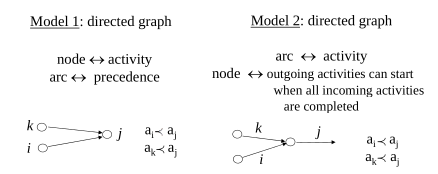
\includegraphics[width = \textwidth]{./images/Precedence.png}
				\end{figure}

			\paragraph{Minimum spanning trees and optimal message passing}
				Wecan model a network of peers as a weighted graph where each node is a peer and each edge has associated (as the weight) the probability of interception of a message along that channel. The problem of finding a broadcasting tree with the minimum interception probability is a minimum spanning tree problem. We call $p_{i\, j}$ the probability of interception between nodes i and j, and the objective function of the problem is simply
				\begin{equation}
					max\, \prod_{i, j \in T} (1 - p_{i\, j})
				\end{equation}

			\paragraph{O($n^2$) Prim's algorithm formulation}
				This formulation of the algorithm uses as data structure a vector that's long as the number of nodes. Each entry in the vector is numbered as the associated node, so that this vector represents \textit{the predecessors} at the end of the algorithm. At startup, it will be filled with the ID of the starting node. At each iteriation, the vector is updated where a path is found that decreases the cost of a node (if node 3 is reachable through node 2 with a decreasing-cost edge, the enntry in position 3 will be updated to 2).
				\begin{figure}[H]
					\centering
					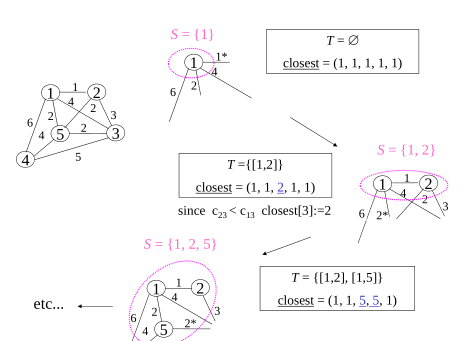
\includegraphics[width = \textwidth]{./images/Prim.png}
				\end{figure}

			\paragraph{DAGs and Gantt charts}
				Given the output of the Critical Path Method, we can build a visual chart that represents the actual parallelism and slack of each activity in a more intuitive way. Example:
				\begin{figure}[H]
					\centering
					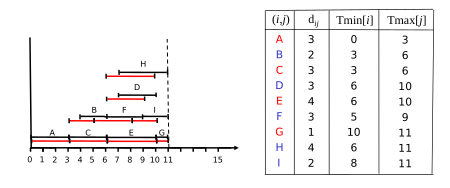
\includegraphics[width = \textwidth]{./images/Gantt.png}
				\end{figure}

			\paragraph{Network flow and matching problems}
				The already discussed task-engineers problem can be seen as a network flow problem, where we're trying to maximize the flow between the first half (the engineers) and the second half of the nodes (the tasks). Note that the graph must be \textit{bipartite}.\\
				The idea is to add a fake initial and final node to have a connected graph (the weights of the additional edges must be all equal) and then finde the maximum possible flow through the network: this will highlight the best combination of assignements for the engineers.


		\subsection{Integer Linear Programming}
			\paragraph{Knapsack problem}
				We have to determine a subset of the carriable objects that fit into the knapsack and maximize the value.
				\begin{equation}
					\begin{cases}
						n \text{ objects} \\
						p_j \text{ profit for object } j \\
						v_j \text{ volume for object } j \\
						b \text{ maximum sack capacity}
					\end{cases}
				\end{equation}
				we define binary variable $x_j$ that indicates if we chose to pick object $j$. The problem has a very easy to understand objective function and feasible region:
				\begin{equation}
					\begin{cases}
						\max(\sum_{j=1}^n p_j x_j) \text{ maximize profit}\\
						\sum_{j=1}^n v_j x_j \leq b \text{ maximum volume constraint}\\
						x_j \in \{0, 1\} \forall j \text{ decision variable constraint}
					\end{cases}
				\end{equation}

			\paragraph{Transportation problem}
				Classic offer-demand-constraint problem, characterized by:
				\begin{equation}
					\begin{cases}
						m \text{ production plants} \\
						n \text{ clients} \\
						c_{ij} \text{ transportation cost from } i \text{ to } j \\
						p_i \text{ production capacity for plant } i \\
						d_j \text{ demand of client } j \\
						q_{ij} \text{ maximum amount that can be transported on that road}
					\end{cases}
				\end{equation}
				Again a very intuitive problem to solve: we must minimize the total transportation cost satisfying the demands and without exceeding the transportation limit of roads. We use decision variable $x_{ij}$ to describe the amount of product transported from plant to clinet.
				\begin{equation}
					\begin{cases}
						\min(\sum_J ( \sum_I (c_{ij} \times x_{ij}))) \\
						\sum_I (x_{ij}) \geq d_j \\
						\sum_J (x_{ij}) \leq p_i \\
						0 \leq x_{ij} \leq q_{ij} \forall (i, j)
					\end{cases}
				\end{equation}


\end{document}
